\chapter{Artificial Neural Networks}
\section{Artificial Neuron}
Our brain is composed by biological neurons and an artificial neuron (or AN) is a representation of it. Every AN can gather signals from other nurons or from the environment, and after an elaboration it transmits another signal to all the other ANs that are connected to it \cite{engelbrecht2007computational}. A rapresentation of AN is depicted in \ref{fig:artificial_neuron}. \\
Each connection to the artificial neuron has a numerical weigth associated to it in which the input signal is hold back. The value of the weight can be either positive or negative. In most cases, the sums of each node are weighted and then given as input to a \textit{non-linear} function called \textbf{transfer function} or \textbf{activation function} \cite{artificial_neuron_wiki}. The activate function defines the output value of the node and typically, the \textit{Step Function}, \textit{Sigmoid Function} and a \textit{Softmax Function} are the most used.

\begin{figure}[!ht]
    \centering
    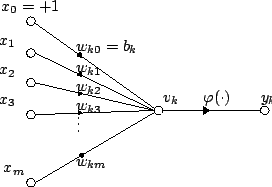
\includegraphics[scale=0.5]{Figures/artificial_neuron.png}
    \caption{Representation of an Artificial Neuron \cite{artificial_neuron_wiki}}
    \label{fig:artificial_neuron}
\end{figure}

\noindent From the mathematical point of view, we can define an artificial neuron as follow: \\
given $m+1$ inputs with signals from $x_1$ to $x_m$ and weights values from $w_0$ to $w_m$. The \textit{bias} is then defined by the input $x_0$ in which a value of 1 will be assigned. The bias value allows us to \textit{shift} the curve of the activation function to a certain direction and it is defined with $w_{k0} = b_k$ \cite{artificial_neuron_wiki}. \\
The output of the AN is:

\begin{equation*}
    y_k = \varphi \left ( \sum_{j=0}^{m} w_{kj} x_j \right )
\end{equation*}

\section{Network Function}
When there are many aritificial neurons interconnected between each other in the different layers, we form a \textit{network}. \ref{fig:ann} shows an example of ANN where the \textbf{inputs} are represented by the first layer in which they send data through the connection to the second group of neuron. The connection between two neuros is called \textit{synapses} where the \textbf{weigth} is stored. The second layer is connected to the third one that represents the \textbf{output} of the network. There can be multiple stratums between the inputs and the outputs and these are called \textit{hidden layers}. \\

\begin{figure}[!ht]
    \centering
    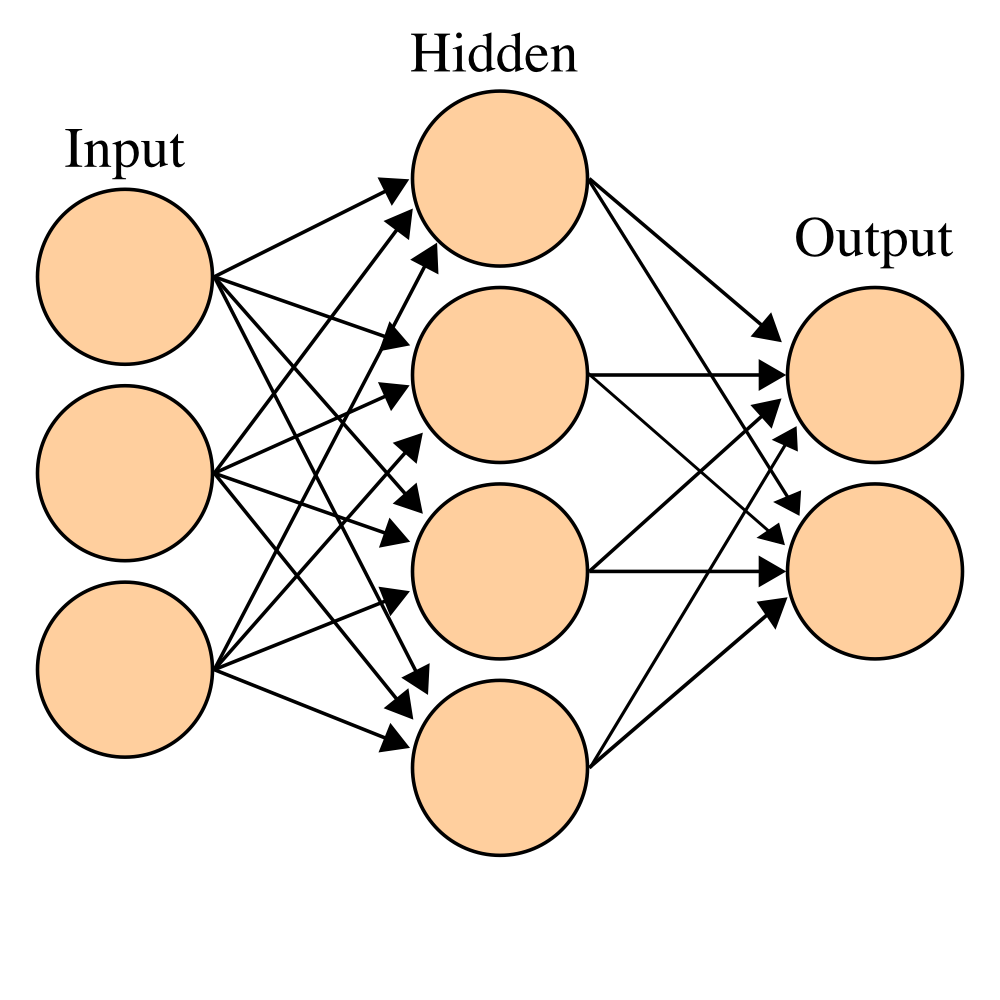
\includegraphics[scale=0.15]{Figures/ann.png}
    \caption{Example of ANN \cite{ann_wiki}}
    \label{fig:ann}
\end{figure}

\vspace*{0.33in}

\noindent Typically, a neural network is defined by three factors:
\begin{itemize}
    \item[1] How the different layers are interconnected
    \item[2] How the the weights are updated (learning process)
    \item[3] How the neuron's input value is converted to its output activation (activation function)
\end{itemize}

\section{Learning}
For every application the design of a neural network is different and after it has structured, the NN is ready to be trained. The first step is the initialization of the weigths. Normally they are initialized with random values, although, in \cite{yam2000weight} they developed a method to \textit{``determining the optimal initial weights of feedforward neural networks based on the Cauchy's inequality and a linear algebraic method''}. More, in \cite{fernandez2001weight} they tested seven different weights' initialization for twelve different problems. Thus, even the initialization of the connections values is application-dependant. \\
\noindent The learning paradigms can be grouped in three major categories: \textbf{supervised}, \textbf{unsupervised} and \textbf{reinforcement learning}.

\subsubsection{Supervised Learning}
This learning technique is the task of inferring a function from labeled training data \cite{sup_learn_wiki} \cite{mohri2012foundations}. The set responsible for training the model is composed by \textit{training examples} in which every sample consists of an \textit{input object} and a \textbf{desidered} \textit{output value}. What the algorithms does is to analyze the train dataset and produce an inferred function that will be used to map the new examples \cite{sup_learn_wiki}. Basically, the algorithm can be seen as \textit{learning} with a \textit{teacher}, in the sense that the there is costantly a feedback on the status of the application.

\subsubsection{Unsupervised Learning}
While in supervised learning, the system has a desidered output given from the training dataset, in the unsupervised paradigm, the system has to learn to estimate the right output given a new input \cite{ghahramani2004unsupervised}. In \textit{classification}, this output is a class label whereas in \textit{regression} is a real number. There are several ways to model this kind of learning system. \textit{Clustering}, using \textit{Self-Organizing Maps}, \textit{K-means} or \textit{hierachical clustering} are among the most famous approaches.

\subsubsection{Reinforcement Learning}
In reinforcement learning, the system takes actions to interact with its own environment. Each action will affect the state of the environment in which will produe a result in a form of either \textit{reward} or \textit{punishment}. The goal of this learning paradigm is to learn which is the best sequence of actions that maximises the rewards or minimises the punishments. There are quite a few approaches to find the best sequence of actions. The most famouse are \textit{Monte Carlo methods}, \textit{Temporal Difference methods} and \textit{Direct Policy search methods}.

\section{Multilayer Perceptron}
A multilayer perceptron (MLP) is a feedforward artificial neural network model that maps sets of input data onto a set of appropriate outputs. An MLP consists of multiple layers of nodes in a directed graph, with each layer fully connected to the next one. Except for the input nodes, each node is a neuron (or processing element) with a nonlinear activation function. MLP utilizes a supervised learning technique called backpropagation for training the network. MLP is a modification of the standard linear perceptron and can distinguish data that are not linearly separable.

\subsection{Activation Function}


\subsection{Layers}


\subsection{Learning through Backpropagation}


\subsubsection{Gradient Descent}
